\section{Evaluation}


\begin{figure}[htb!]
\begin{center}
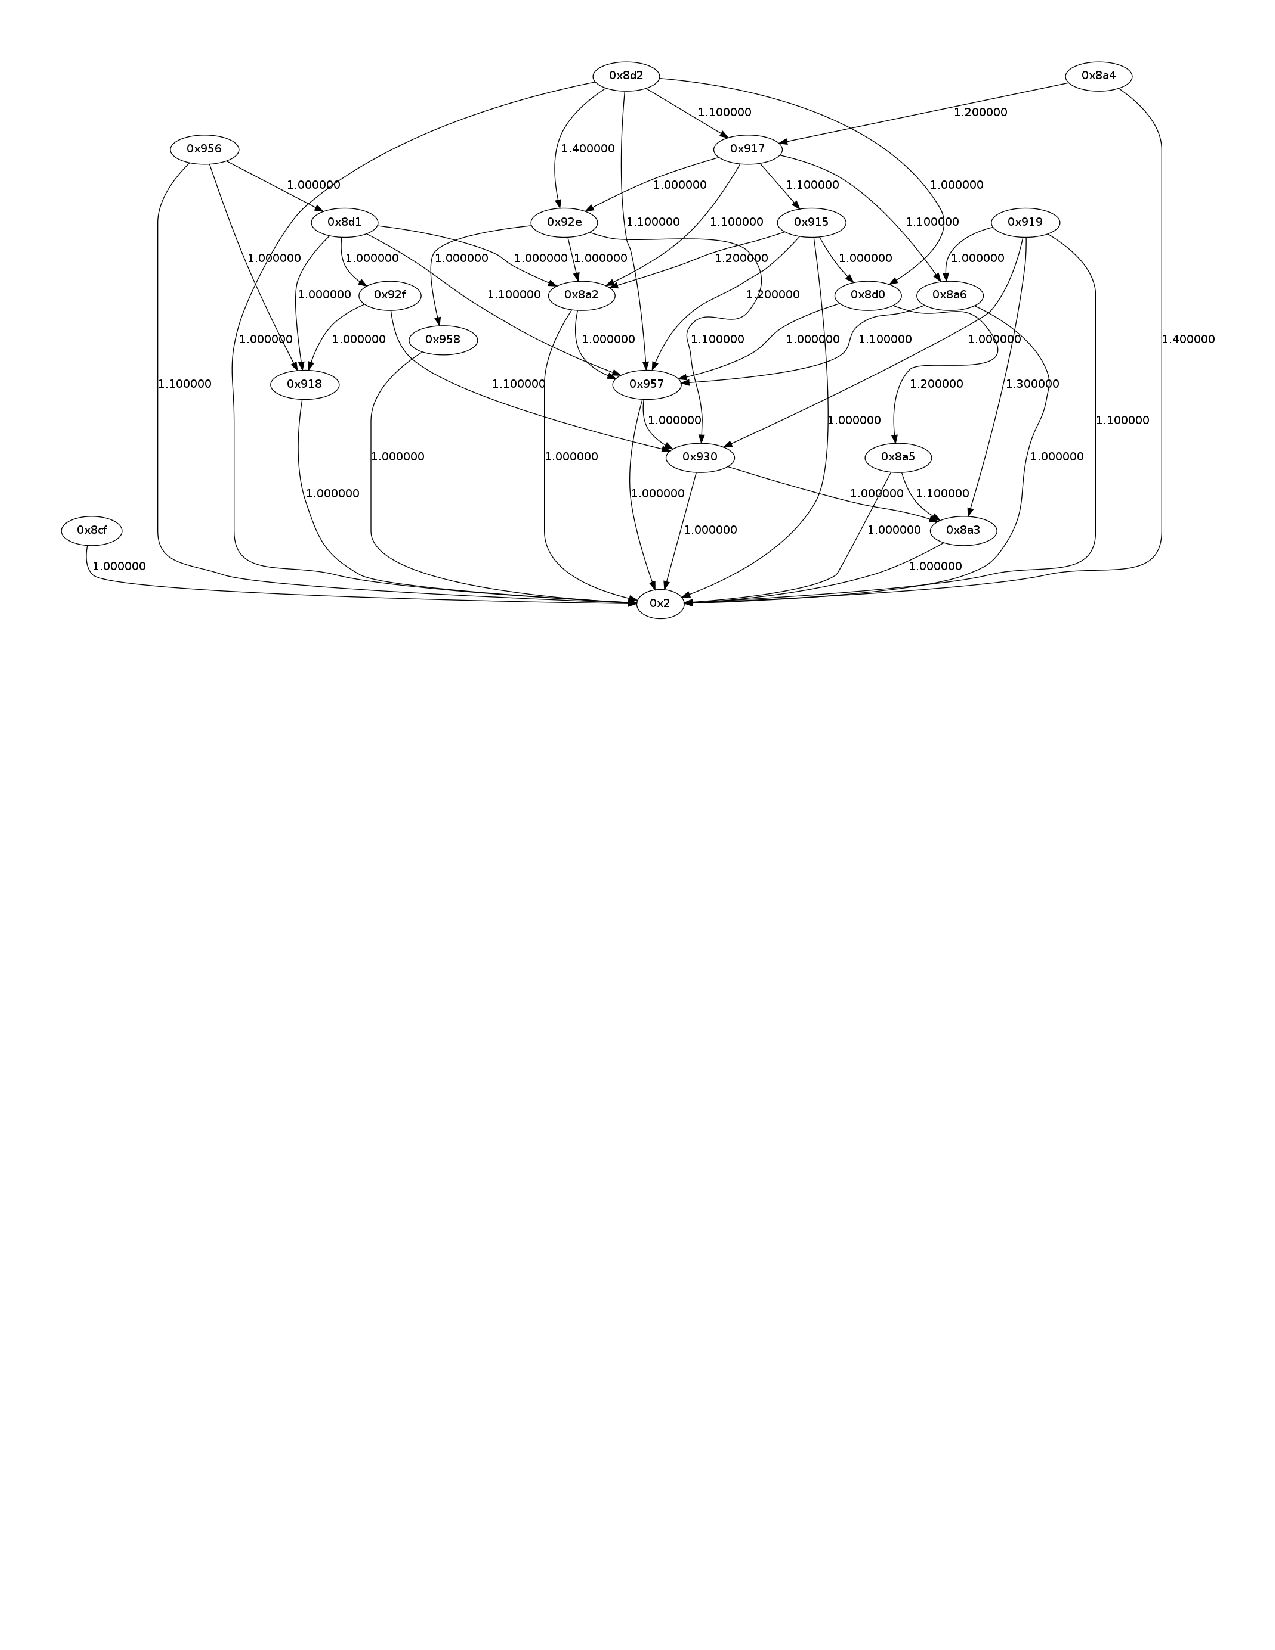
\includegraphics[scale=0.4]{figs/acmenetwork_SDH_4F}
\caption{}
\label{fig:acmenetwork_SDH_4F}
\end{center}
\end{figure}


\subsection{Prefetching}

\begin{algorithm}
\caption{Prefetch Loop}
\label{alg:prefetcher}
	\begin{algorithmic}
	\While {true}
	\If {connected and active}
	    \State $req\gets [t_{i-n}, OP_R]$
	    \State $resp\gets $ send($req$)=$[t_{i-k}, OP_R],\dots, [t_{now}, OP_R]; $ 
	    \State $n >= k$
	    \For {$j = 1 \to size(resp)}$
	    	\State $op \gets$ $resp[j]=[t_{i-k+e}, OP_R]$
	    	\State apply($op$)
	    \EndFor
	\EndIf
	\If {active}
		\State Sleep for 10 minutes
	\Else
		\State Sleep for 1 hour
	\EndIf
	\EndWhile
	\end{algorithmic}
\end{algorithm}



\begin{table}
\label{tab:qrscans}
\begin{center}
  \begin{tabular}{| r | c  c | }
    \hline
    {\bf No. nodes } & {\bf Fetch time (sec) } & {\bf Std. Error (sec)} \\ \hline
    1 & 0.8902 & 0.0756 \\ \hline
    10 & 5.7342 & 1.7087 \\ \hline
    100 & 52.3145 & 14.1146 \\ 
    \hline
  \end{tabular}
\caption{Shows the time to fetch nodes based on the size of the fetch.  The fetch time
increased linearly with the number of nodes.  Caching maintain fetch time near
that of fetching a single node.  A callback is used when cache is invalidated.}
\end{center}
\end{table}

\subsection{Log dump measurements}


\subsection{Global transaction manager}
Maybe we include another table that talks about the trace we ran through and the conflict times, etc.

\begin{itemize}
\item Forwarding
\item Conflict resolution
\end{itemize}




% The main driver for the EnergyLens work is to explore the fundamental challenges related to:

% \begin{enumerate}
% \item Tracking people and objects.
% 	\begin{itemize}
% 	\item Through local crowd-sourcing of the tasks to building occupants
% 	\end{itemize}
% \item Maintaining consistency between the relationship between physical items and the entity-relationship graph that represents it.
% \item Providing real-time statistics, information, and processing of energy data related to the building environment.

% 	\begin{itemize}
% 	\item With respect to the occupants
% 	\item with respect to spaces
% 	\item Maintaining security and privacy
% 		\begin{itemize}
% 		\item specifically with respect to personal data and control
% 		\end{itemize}
% 	\end{itemize}

% \end{enumerate}


